\documentclass[a4paper,12pt]{article}

%-------------------------------------------------------------------------------
% Paquetes
%-------------------------------------------------------------------------------

% Permite reconocer acentos
\usepackage[utf8]{inputenc}
% Salida correcta para copiar desde el PDF
\usepackage[T1]{fontenc}
% Anchura correcta de los márgenes
\usepackage{a4wide}
% Usar la fuente Latin Modern
\usepackage{lmodern}
% Establece el idioma del documento
\usepackage[spanish]{babel}
% Permite instertar imágenes
\usepackage{graphicx}
% Control de los párrafos
\usepackage{parskip}
% Modifica el índice
\usepackage[nottoc,numbib]{tocbibind}
% Diferentes tamaños de letra
\usepackage{anyfontsize}
% AMS
\usepackage{amsmath, amsfonts, amssymb}
% Mejor apariencia del texto
\usepackage{microtype}
% Personalizar los encabezados y pies de página
\usepackage{fancyhdr}
% Mejores tablas
\usepackage{booktabs}
% Hipervínculos
\usepackage[colorlinks=false, pdfborder={0 0 0}]{hyperref}

\usepackage[table,xcdraw]{xcolor}

% Información del Documento
\title{
\huge \bfseries Memoria
}
\author{David Gasquez}
\date{}

% Indentar los párrafos
\setlength{\parindent}{\baselineskip}
\linespread{1.25}

%-------------------------------------------------------------------------------
% Inicio del Documento
%-------------------------------------------------------------------------------

\begin{document}

% Incluir la portada
\begin{titlepage}

% Comando para dibujar las líneas horizontales
\newcommand{\HRule}{\rule{\linewidth}{0.7mm}}

% Centrar todo
\center 
 
%----------------------------------------------------------------------------------------
% Sub-títulos
%----------------------------------------------------------------------------------------

\textsc{\Huge Visión Por Computador}\\[2.5cm] 
\textsc{\LARGE Proyecto Final}\\[3cm]


%----------------------------------------------------------------------------------------
% Título
%----------------------------------------------------------------------------------------

\HRule \\[1cm]
{\fontsize{55}{60}\selectfont \sffamily Memoria}\\[0.6cm] 
\HRule \\[8.2cm]
 

%----------------------------------------------------------------------------------------
% Información adicional
%----------------------------------------------------------------------------------------

\begin{minipage}{0.4\textwidth}
\begin{flushleft} \large
David \textsc{Gasquez}\\ % Your name
\texttt{76421093M}\\
davidgasquez@gmail.com
\end{flushleft}
\end{minipage}
~
\begin{minipage}{0.4\textwidth}
\begin{flushright} \large
\end{flushright}
\end{minipage}\\[4cm]


\end{titlepage}



%-------------------------------------------------------------------------------
% Índice
%-------------------------------------------------------------------------------
\pagestyle{empty}
\renewcommand{\contentsname}{\centering Índice}
\tableofcontents
\newpage


%-------------------------------------------------------------------------------
% Estilo de las cabeceras y de los piés de página
%-------------------------------------------------------------------------------

\pagestyle{fancy}
\cfoot{\thepage}
\rhead{}
\renewcommand{\headrulewidth}{0pt}
\renewcommand{\footrulewidth}{0.4pt}
\renewcommand{\headheight}{15pt}


%-------------------------------------------------------------------------------
% Contenido
%-------------------------------------------------------------------------------

\section{Descripción del Problema}

\subsection{Introducción}

El problema al que nos enfrentamos se trata de la clasificación automática de
la categoría a la que pertenece un objeto o varios. Es uno de los temas más 
activos en investigación actualmente. Actualmente el reconocimiento de la
instancia de un objeto en particular está bastante asentado. El problema
pués, se trata de reconocer la categoría a la que pertenece un objeto en
cuestión y no de que objeto específico se trata. La correcta categorización 
de un objeto nos proporciona información adicional sobre el mismo, como puede
ser su uso.

El enfoque de esté trabajo va a ser la clasificación de objetos en 101 
distintas categorías usando la base de dátos pública del
California Institute of Technology.

La clasificación en nuestro caso será indicar la presencia o nó de una categoría
en una imagen dada. Asignar una categoría a una imagen presenta varios 
problemas:
\begin{itemize}
  \item Diferencias en el aspecto del objeto
  \item La imagen puede tomarse en distintas condiciones,posiciones\ldots
  \item Puede ser subjetivo, dependiendo del observador
\end{itemize}

\subsection{Procedimiento}
\begin{enumerate}
  \item Extraer un número considerable de descriptores SIFT(entre 50.000 y 
  100.000) de un conjunto de imágenes cualesquiera
  \item Realizar entre 200 y 1500 clústeres usando la técnica KNN con los
  descriptores SIFT
  \item Obtener de cada categoría un conjunto de imágenes de entrenamiento, de
  las cuales obtenemos los descriptores SIFT densos para contrastarlos con los
  clústeres y crear el descriptor de la imagen
  \item Entrenar una máquina de soporte vectorial con dichos descriptores para
  cada clase
  \item Comprobar los resultados con un conjunto de test
\end{enumerate}

\newpage
\section{Implementación}

La implementación del proyecto se ha llevado a cabo en el lenguaje de 
programación C++. También se ha usado scripts bash para facilitar algunas
tareas. 

\subsection{Clustering}

La primera parte ha consistido en realizar un módulo que fuese capáz de leer
imágenes de una carpeta y calcular los descriptores de dichas imágenes.

Los descriptores se han seleccionado uniformemente entre las imágenes y se 
obtienen a partir de la técnica SIFT; Una vez tenemos el vector de imágenes y
el número de descriptores(puntos SIFT) que queremos obtener, realizamos la 
división para obtener el número máximo de descriptores por imágen.

Cuando disponemos del vector con todos los descriptores de las imágenes 
proporcionadas, pasamos a agruparlos usando KNN. Esto se realiza usando
la función \texttt{kmeans()} de OpenCV, dicha función devuelve los centros
de los clústeres que hemos decidido hacer($K$). Los clústeres forman nuestro
vocabulario.

\subsection{Bag Of Words}

Ya tenemos el vocabulario calculado, ahora proseguimos aplicando la técnica
Bag Of Words o Bag Of Features. El objetivo de esta fase es obtener un 
descriptor que represente a cada imagen. El descriptor se puede obtener
realizando los siguientes pasos.

Por cada imagen a la que queremos calcular su descriptor BoW, tenemos que 
obtener una gran cantidad de puntos SIFT(Denso). Con estos puntos SIFT podemos
realizar un histograma(que será nuestro descriptor BoW) comparando cada 
descriptor con nuestro vocabulario para hayar la palabra más cercana que 
dé el voto a dicha ``palabra''.

Cuando hemos terminado con una imagen deberíamos tener un vector con $K$ 
posiciónes y en cada posición el número de veces que un descriptor SIFT de la 
imagen original ha quedado cerca de la ``palabra''. Para que la clasificación
funcione bien con las máquina de soporte vectorial, tenemos que normalizar
el histograma resultante. En este paso se ha utilizado la función de OpenCV
\texttt{BOWImgDescriptorExtractor::compute}\footnote{ La documentación y 
descripción breve del funcionamiento puede encontrarse en
\url{http://docs.opencv.org/modules/features2d/doc/object_categorization.html}

La implementación se puede consultar en 
\url{https://github.com/Itseez/opencv/blob/master/modules/features2d/src/bagofwords.cpp}
} que sigue el esquema general para calcular el descriptor según la técnica
\emph{Bag of Visual Words}.

Este es el descriptor que nos sirve para identificar cada imagen. Dicho esto
procedemos a entrenar una máquina de soporte vectorial con los descriptores de
un conjunto de imágenes que representen el mismo ``concepto''.  Cada conjunto
de imágenes será una categoría. 

\subsection{Test}

La última parte se trata de comprobar como han sido de efectivos nuestros 
descriptores, para ello calculamos la matriz de confusión, que nos ofrece una 
forma rápida y fácil de ver los resultados.

Se han separado las imágenes de la base de datos Caltech101 en dos grupos.
Un grupo con el 70\% de las imágenes de cada categoría que se usa para el 
entrenamiendo de la SVM. Y otro grupo con las imágenes de test para poder
realizar la matriz de confusión.

También se ha creado una ejecutable para poder clasificar imágenes aisladas.
La clasificación se ha limitado a las 101 clases de la base de datos. No se 
proporciona la opción de ``otros'' que puede ser interesante si queremos un 
clasificador general. Si se quisiera añadir esta opción, solo habría que 
establecer un humbral a partir del cual los objetos no son de ninguna clase 
conocida.

\newpage
\section{Experimentación}

Antes de empezar, vamos a crear un subconjunto de clases aleatorias para poder
realizar los test en un tiempo razonable\footnote{Dado el tamaño de la base de 
datos, no se ha conseguido completar una ejecución completa con las 101 clases
que disponíamos al principio, con 10 clases, el tiempo de ejecución es de 
20 minutos}. Una vez seleccionadas ejecutamos el 
clasificador BoW y comprobamos con el conjunto de test. El porcentaje 
de acierto es del $75,73\%$ con 50.000 descriptores y 500 clústeres. Los 
parámetros del matcher, descriptor y extractor son los parámetros por defecto.
Se está usando un matcher por fuerza bruta(L2 por defecto), un detector de
puntos de interés denso\footnote{\url{http://docs.opencv.org/modules/features2d/doc/common_interfaces_of_feature_detectors.html\#densefeaturedetector}}, este detector genera varios niveles de puntos de 
interés que se reparten en una cuadrícula por la imágen. Y por último, el 
extractor de puntos es SIFT. 

La matriz de confusión de la ejecución es la siguiente
\begin{table}[h]
\centering
\begin{tabular}{c|c|c|c|c|c|c|c|c|c|c|}
\cline{2-11}
 & \textbf{1} & \textbf{2} & \textbf{3} & \textbf{4} & \textbf{5} & \textbf{6} & \textbf{7} & \textbf{8} & \textbf{9} & \textbf{10} \\ \hline
\multicolumn{1}{|c|}{\textbf{1}} & \cellcolor[HTML]{dddddd}{\color[HTML]{343434} 3} & 1 & 0 & 0 & 1 & 0 & 1 & 3 & 1 & 0 \\ \hline
\multicolumn{1}{|c|}{\textbf{2}} & 1 & \cellcolor[HTML]{dddddd}1 & 1 & 1 & 0 & 2 & 0 & 3 & 2 & 1 \\ \hline
\multicolumn{1}{|c|}{\textbf{3}} & 0 & 7 & \cellcolor[HTML]{dddddd}9 & 0 & 0 & 1 & 0 & 2 & 0 & 0 \\ \hline
\multicolumn{1}{|c|}{\textbf{4}} & 0 & 0 & 0 & \cellcolor[HTML]{dddddd}11 & 1 & 1 & 0 & 1 & 0 & 0 \\ \hline
\multicolumn{1}{|c|}{\textbf{5}} & 1 & 1 & 4 & 1 & \cellcolor[HTML]{dddddd}4 & 1 & 2 & 3 & 0 & 0 \\ \hline
\multicolumn{1}{|c|}{\textbf{6}} & 0 & 0 & 0 & 2 & 0 & \cellcolor[HTML]{dddddd}19 & 1 & 2 & 0 & 0 \\ \hline
\multicolumn{1}{|c|}{\textbf{7}} & 1 & 0 & 3 & 0 & 0 & 3 & \cellcolor[HTML]{dddddd}10 & 1 & 0 & 0 \\ \hline
\multicolumn{1}{|c|}{\textbf{8}} & 0 & 0 & 0 & 0 & 1 & 1 & 0 & \cellcolor[HTML]{dddddd}128 & 0 & 0 \\ \hline
\multicolumn{1}{|c|}{\textbf{9}} & 0 & 0 & 1 & 0 & 0 & 3 & 0 & 0 & \cellcolor[HTML]{dddddd}13 & 0 \\ \hline
\multicolumn{1}{|c|}{\textbf{10}} & 0 & 0 & 0 & 0 & 0 & 0 & 0 & 3 & 0 & \cellcolor[HTML]{dddddd}8 \\ \hline
\end{tabular}
\end{table}

Podemos ver que en la fila 8, que representa a la categoría de caras, al tener 
muchas muestras y clasificarlas bien en su mayoría, está ayudando a que el ratio
de acierto sea bueno. En la mayoría de las categorías, se predice más veces 
correctamente que incorrectamente, salvo en la segunda categoría, que representa
la categoría de ``hormigas''.

Vamos a ir analizando los cambios en los parámetros de cada módulo, para 
intentar conseguir el máximo de aciertos con nuestras 10 clases.

\subsection{Creación del Vocabulario}
Vamos a comenzar viendo el impacto del número de descriptores a la hora de
crear el vocabulario en la tasa de aciertos, que será nuestra medida a 
optimizar. Se ejecuta con un rango desde 50.000 descriptores hasta 100.000 y 
siempre creando 500 clústeres(palabras visuales). 

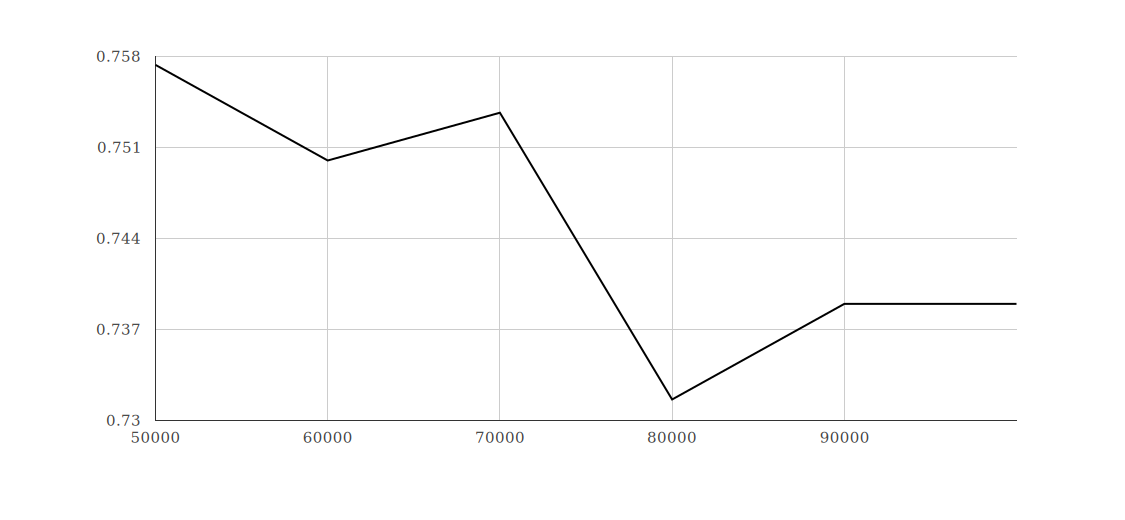
\includegraphics[width=15cm]{charts/descriptors}

Los resultados los podemos observar en la gráfica anterior. Parece que el número
de descriptores que necesitamos no afecta de forma significativa a el 
porcentaje de aciertos. Esto puede ser debido a que con los 50000 descriptores
que tenemos al principio ya cubrimos el rango de ``palabras importantes'' para 
luego agrupar. 

Vamos a ver si mantenemos fijo el numero de descriptores a 50.000
y vamos alterando desde los 200 a los 1500 clústeres, como evoluciona el ratio
de aciertos.

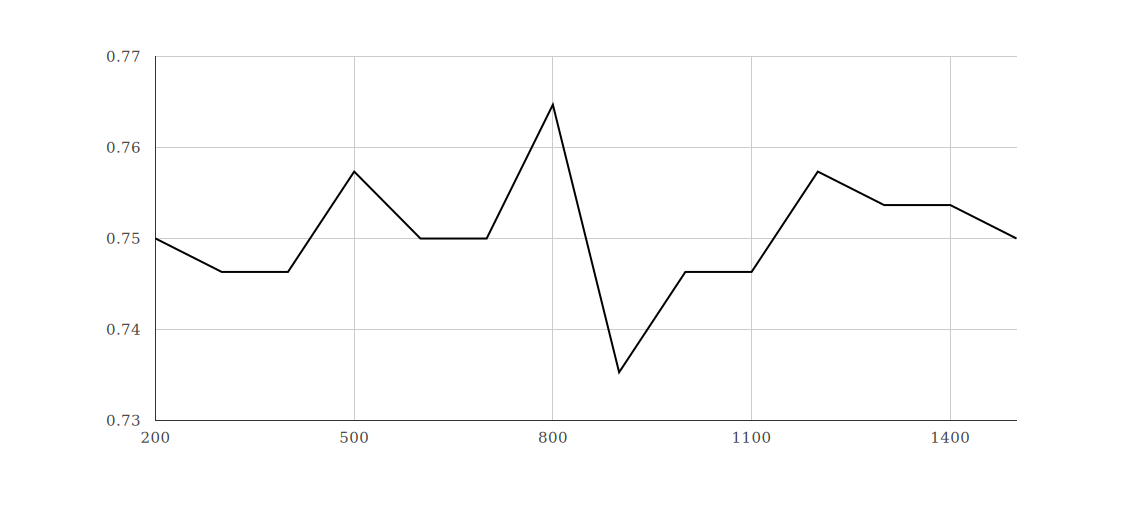
\includegraphics[width=15cm]{charts/clusters}

Al igual que pasaba anteriormente, al variar el número de clústeres tampoco 
parece haber impacto significativo en las predicciones. De nuevo, es posible que
con un número de clústeres elevado, muchos no sean importantes y nunca sean
``votados''.

Ya que no existe gran diferencia entre las salidas que proporciona el programa,
cuando se varía tanto descriptores como número de clústeres, vamos a tomar como
referencia; número de descriptores 50.000 y 800 como número de clústeres para
proceder a experimentar alterando los valores o el tipo de matcher, detector y
extractor. El valor que tomamos como base después de esta experimentación es
un ratio de 76,473\%

\subsection{Bag of Words}

Primero vamos a ver el efecto del matcher. Para ello ejecutamos con el mismo
\texttt{BFMatcher}, pero cambiando de \emph{norm} \texttt{L2} a \texttt{L1}. El resultado es la bajada de
2 puntos en el resultado final 74,256\% , la otra opción es \texttt{NORM\_HAMMING}
pero, tal como dice la documentación, \texttt{L2} y \texttt{L1} son los que se usan en SIFT.

Mantenemos pués el mismo matcher(fuerza bruta con \texttt{L2}).
Actualmente se está usando el detector de puntos de interés denso con los 
parámetros por defecto, esto es, detectando puntos a una sola escala y con un
tamaño de celda de 6. 

Ejecutando el mismo detector, pero cambiando el tamaño de  celda de 6 a 3, 
mejoramos hasta 76,89\%. No es una mejora significativa y el tiempo
de cómputo se ha visto aumentado, por lo que seguimos intentando mejorar 
cambiando de detector. 

Con el detector \texttt{FAST} se obtiene

FAST - 79.77
SIFT - 71.16
SURF - 81.25
ORB - 72.42
BRISK - 64.33
MSER - 76.10
GoodFeaturesToTrackDetector - 77.57
Dense - 76.89

PyramidAdaptedFeatureDetector FastFeatureDetector 83.45
% CAMBIOS EN EL EXTRACTOR

\subsection{Otras mejoras}

% CITAR QUE PODRIAN HACERSE CAMBIOS EN LA SVM
Otro de los cambios importantes que podrian aplicarse para mejorar el 
rendimiento del predictor es configurar la máquina de soporte vectorial y no 
usar parámetros automáticos, así puede que las predicciones sean más certeras.

También es posible realizar cambios en la implementación de los descriptores e 
implementar descriptores piramidales en los que se evaluan los puntos relevantes
a varias escalas y se concatenan los ``histogramas''.

% CITAR QUE PODRIAN CAMBIARSE LA FORMA DE COMPUTAR LOS DESCRIPTORES Y HACERLOS PIRAMIDALES 

\newpage
\section{Resultados}

% COMENTAR LOS RESULTADOS GENERALES

% COMENTAR LA DIFICULTAD DE LEER LA BASE DE DATOS

% COMENTAR LOS RESULTADOS QUE SE OBTIENEN CON OTRAS CATEGORIAS, MAS Y MENOS

\newpage
\section{Conclusiones}

El procedimiento realizado posee ventajas como la facilidad de implementación
y unos resultados asequibles, aunque con una base de datos grande se necesita
mucha potencia de cómputo para que sea efectivo. La desventaja de la potencia o 
tiempo de cómputo es importante en este problema ya que lo que se busca es 
aprender el mayor número de categorias posibles para poder etiquetar un 
repertorio más amplio. 

En los últimos meses se han dado a conocer varios estudios que usan diversas 
técnicas con el mismo propósito, saber lo que hay en una fotografía. Una de las
técnicas con más potencial es el uso de redes neuronales para la clasificación
\footnote{\url{http://static.googleusercontent.com/media/research.google.com/en//pubs/archive/40814.pdf}},
y desde hace poco el uso de lo que se denomina \emph{deep learning}. Empresas como
\url{http://www.clarifai.com/} ofrecen online su herramienta como demostración
de lo que es posible alcanzar usando su tecnología.

Avanzar en este campo implica un gran impacto en la vida cotidiana en un futuro
cercano, en donde automáticamente se puedan clasificar imágenes según su 
contenido, o bien filtrar para realizar búsquedas más rápidamente. El aporte de 
conocimiento que otorga la correcta categorización de un objeto o imagen es, 
hoy en día, un valor importante en el mundo empresarial. 

Se ha facilitado el código online en la plataforma
\href{https://github.com/DavidGasquez/category-recognition}{\texttt{Github}},
además, se  proporcionan las herramientas e instrucciones necesarias para que 
personas sin conocimiento en visión por computador puedan recrear el experimento 
de forma sencilla, y clasificar imágenes con la ejecución del módulo 
independiente que lee el vocabulario y máquina de soporte vectorial creadas 
anteriormente con toda la base de datos(juntando de nuevo test y entrenamiento)
para clasificar nuevas imágenes.

%-------------------------------------------------------------------------------
% Bibliografía
%-------------------------------------------------------------------------------

\newpage
\begin{thebibliography}{99}

\bibitem{VCBOW01}
 \textbf{Visual Categorization with Bags of Keypoints}. 
 \emph{Gabriella Csurka, Christopher R. Dance, Lixin Fan, Jutta Willamowski, Cédric Bray.}
 2004 \url{https://www.cs.cmu.edu/~efros/courses/AP06/Papers/csurka-eccv-04.pdf}

\bibitem{OpenCV} \url{http://docs.opencv.org/modules/features2d/doc/features2d.html}

\bibitem{Blog} \href{http://www.morethantechnical.com/2011/08/25/a-simple-object-classifier-with-bag-of-words-using-opencv-2-3-w-code/}
{http://www.morethantechnical.com/ - A simple object classifier with Bag-of-Words using OpenCV 2.3}

\end{thebibliography}



\end{document}
